\documentclass[english]{article}
\usepackage[T1]{fontenc}
\usepackage[latin9]{inputenc}
\usepackage{geometry}
\usepackage{graphicx}
\geometry{verbose,tmargin=2cm,bmargin=2cm,lmargin=2cm,rmargin=2cm}
\usepackage{color}
\usepackage{babel}
\usepackage{bm}
\usepackage{amsmath}
\usepackage{amsthm}
\usepackage{amsfonts}
\usepackage{amssymb}
\usepackage{parskip}
\usepackage{amsfonts}
\usepackage[unicode=true,pdfusetitle,
 bookmarks=true,bookmarksnumbered=false,bookmarksopen=false,
 breaklinks=false,pdfborder={0 0 1},backref=page,colorlinks=true]
 {hyperref}

\makeatletter
%%%%%%%%%%%%%%%%%%%%%%%%%%%%%% Textclass specific LaTeX commands.
\usepackage[natbibapa]{apacite}
\theoremstyle{plain}
\newtheorem{theorem}{Theorem}
\newtheorem{lemma}{Lemma}
\newtheorem{definition}{Definition}

%%%%%%%%%%%%%%%%%%%%%%%%%%%%%% User specified LaTeX commands.

\newcommand{\E}{\mathbb{E}}
\usepackage{pdfsync}

\DeclareMathOperator{\conv}{conv}
\DeclareMathOperator{\st}{s.t.}
\DeclareMathOperator{\dom}{dom}
\DeclareMathOperator{\im}{im}
\DeclareMathOperator{\Ne}{Ne}
\DeclareMathOperator{\sign}{sign}
\DeclareMathOperator{\Var}{Var}
\DeclareMathOperator{\Cov}{Cov}
\DeclareMathOperator{\diag}{diag}
\DeclareMathOperator{\vvec}{vec}
\DeclareMathOperator{\pa}{pa}
\DeclareMathOperator{\repmat}{repmat}

\def\ci{\perp\!\!\!\perp}

\makeatother

\begin{document}

\title{Expanding Compressed Learning}

\author{Kevin Shi and Kui Tang}
\date{14 December 2015}
\maketitle
\begin{abstract}
Compressed sensing can offer fast and simple techniques for machine learning in high dimensional space. Recently, \citet{Calderbank09} have shown that the RIP$_2$ property of a measurement matrix allows us to train linear support vector machines on compressed measurements directly, rather than recovering a high dimensional sparse vector and working in that space.
They bound the difference of the error of a classifier trained on low-dimensional samples vs. the error of the best classifier on the high-dimensional space by a factor that depends on the data radius, regularization, and the RIP $\epsilon$ parameter.
We show that nearly the same bounds hold for support vector regression (i.e. continuous labels), and for nonlinear models using the squared exponential kernel, though by an exponential factor.
Next we explore a new nonnegative randomized RIP construction using Poisson random variables.
This offers an alternative to the standard Gaussian and Bernoulli RIP matrices, and may be step in the direction towards constructing expander graph RIP matrices.
\end{abstract}

\section{Introduction}

Compressed sensing is based off of two fundamental ideas.
First is constructing an $m \times n$ \emph{measurement matrix} $A$ which satisfies $\emph{restricted isometry property}$ in $L_p$ with parameters $(k,\epsilon)$, abbreviated $\mbox{RIP}_p(k,\epsilon)$.
This means that for any $k-$sparse $x$,
\[
(1-\epsilon)\|x\|_p \le\|Ax\|_p \le (1+\epsilon)\|x\|_p. \label{eq:RIP}
\]
Well-known examples are matrices whose entries are Gaussian $\mathcal{N}(0,\sigma=1/\sqrt{m})$ and ones whose entries are Bernoulli $U(-1/\sqrt{m},1/\sqrt{m})$~\citep{Baraniuk08}.
But these classical constructions have a caveat: being random matrices, the RIP only holds with high probability.
An open question whether we can deterministically construct measurement matrices with RIP.

The next idea is the compressed sensing linear program~\citep{Candes2006}.
Given an input measurement $x$ and a measurement matrix $A$, we seek the solution to
\begin{alignat*}{1}
\min & \left\Vert \widehat{x}\right\Vert _{1}\\
\st & A\widehat{x}=x
\end{alignat*}
Let $y$ be the output of this linear program.
If $A$ satisfying the RIP$_2$ property, then the guarantee is that for any $k$-sparse vector $\tilde{x}$, we have $\|y - x\|_2 \le O(1/\sqrt{k}) \|\tilde{x}-x\|_1$.
In particular this holds for the best $k-$sparse approximation, that is, $\arg\min_{\tilde{x}} \|\tilde{x}-x\|_1$, so this is a rather strong agnostic learning guarantee.
Naturally, we may ask whether the RIP can help use solve learning problems beyond that of $L_1$ signal recovery.

\section{Compressed Learning}
We first review our notations for support vector machines for classification and regression, review existing results, and present our extensions.

\begin{figure}
    \centering
    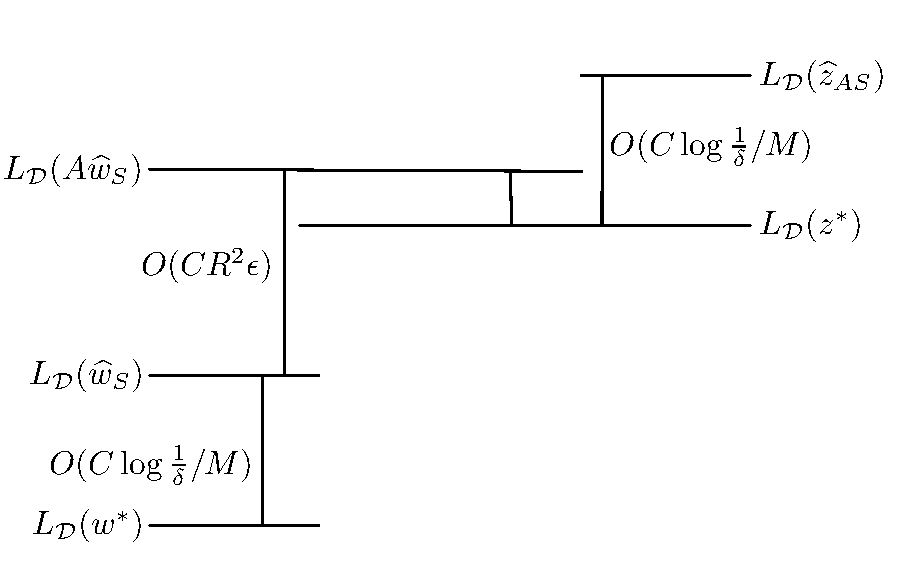
\includegraphics[width=0.6\columnwidth]{bounds_argument_figure.pdf}
    \caption{
Illustration of main argument for compressed learning.
Horizontal lines denote quantities and vertical lines indicate upper bounds.
Note how we can bound the error of the classifier trained on samples from the compressed space $\widehat{z}_{AS}$ to that of the classifier trained on samples from the true space $\widehat{w}_S$ without directly comparing the quantities.
}
    \label{fig:bounds_argument} 

\end{figure}
\subsection{Support Vector Machines}
The training objective for support vector machines is to minimize the hinge loss $H(x,y;w) = \max\{0, 1 - yw^\top x\}$ where $x$ is the input, $y$ is the label, and $w$ is the linear classifier.
We define the true hinge loss on distribution $\cal D$ as $H_{\cal D}(w) = E_{(x_i,y_i) \sim {\cal D}} [1 - y_i w^\top x_i]$
Since our training objective contains a quadratic regularizer, we also define the true regularization as $L(w) = H_{\cal D}(w) + \frac{1}{2C}\left\Vert w \right\Vert$.

The term \emph{support vector} becomes evident when one looks at the dual optimization problem:
\begin{alignat}{1}
\max & \sum_{i}\alpha_{i}-\frac{1}{2}\sum_{ij}\alpha_{i}\alpha_{j}y_{i}y_{j}x_{i}^{\top}x_{j}\\
\text{s.t.} & \forall i\quad0\leq\alpha_{i}\leq C/M
\label{eq:dual_svm}
\end{alignat}
A standard result is then that the SVM classifier $\widehat{w}$ can be written as
\begin{equation}
\widehat{w} = \sum_i \alpha_i y_i x_i
\label{eq:w_dual}
\end{equation}
In fact, many of the $\alpha_i$ will be zero, so $\widehat{w}$ is a sparse convex combination of training points.
The $x_i$'s with positive Lagrange multipliers $\alpha_i$ are the support vectors.

For theoretical analysis, we want to bound $L(\widehat{w})$ for a classifier $\widehat{w}$ trained from an i.i.d. sample of $\cal D$ in terms of the true loss of the best classifier $w^*$ over $\cal D$.
The result is summarized by the following theorem:
\begin{theorem}[\citet{Sridharan08}]
\label{thm:svm-generalization}
Let $\widehat{w}$ be the SVM classifier learned from samples from $\cal D$ and $w^*$ be the best SVM classifier over $\cal D$. Then with probability at least $1 - \delta$ over the training set
\[
L_{\cal D}(\widehat{w}_S) \leq L_{\cal D}(\widehat{w}^*) + O\left(\frac{C \log (1/\delta)}{M}\right)
\]
\end{theorem}

\subsection{Review of Existing Results}
\citet{Calderbank09} show it is possible to merge compressed sensing and learning.
Suppose an $m \times n$ matrix $A$ is $\mbox{RIP}(2k,\epsilon)$.
Suppose our true data $(x_i, y_i) \in \mathbb{R}^n \times \{\pm 1\}$ are labeled $k$-sparse vectors in a high dimensional space $S$, but we only observe compressed samples $(Ax_i,y_i)$ in the compressed space $AS$.
Under these hypotheses, we can of course solve the compressed sensing linear program to recover sparse high-dimensional vectors $\widehat{x}_i$ and train the SVM this space.
Alternatively, we can simply train a classifier on the compressed samples $Ax_i$.
We would like to bound the error introduced by the compressed sensing.
In fact, we can even bound the error of a classifier trained on a sample of compressed data in $AS$ to the best classifier on $S$, even though we do not know any of the $x_i$ directly.
\begin{theorem}[Theorem 3.1 in \citet{Calderbank09}]
\label{theorem:alog} Let $A_{m\times n}$ satisfy $(2k,\epsilon)$-RIP
and let
\[
S=\left\{ (x_{1},y_{1}),\ldots,(x_{M},y_{M})\right\} 
\]
be a training set of size $M$ where each example is sampled i.i.d.
from some distribution ${\cal D}$ in the data domain. Let $\widehat{w}_{S}$
be the sort-margin SVM trained on $S$ and $A\widehat{w}_{S}$ be
the vector in the measurement domain obtained by projecting $\widehat{w}_{S}$.
Then
\[
L_{{\cal D}}(A\widehat{w}_{S})\leq L_{{\cal D}}(\widehat{w}_{S})+O(CR^{2}\epsilon)
\]
where $C\geq\sum_{i}\alpha_{i}$ is an upper bound on sum of the optimal
Lagrange multipliers $\alpha_{i}$ in the dual SVM and $R$ is the
radius of data $x_{i}$.
\end{theorem}

The result follows from chaining together several bounds, illustrated in Figure~\ref{fig:bounds_argument}. One ingredient is the standard generalization bound for SVMs.
The other bound, $L_{\cal D}(A\widehat{w}_S) \leq L_{\cal D}(\widehat{w}_S) + O(CR^2\epsilon)$ can be derived from the following lemma, which states that an RIP matrix $A$ preserves inner products of convex combinations of $k$-sparse vectors:

\begin{lemma}[Theorem 4.4 in~\citet{Calderbank09}]
\label{lemma:their-theorem-44}Let $A_{m\times n}$ be a $(2k,\epsilon)$
RIP matrix and $(x_1,y_1), \ldots, (x_M,y_M)$ and $(x_1',y_1'), \ldots, (x_N',y_N')$ be two labeled datasets. Let $\alpha_1, \ldots, \alpha_M$ and $\beta_1, \ldots, \beta_N$ be nonnegative numbers with $\sum_i \alpha_i \leq C$ and $\sum_j \beta_j \leq D$ for some $C, D \geq 0$. Let
\begin{eqnarray*}
\bm{\alpha} & = & \sum_{i}\alpha_iy_ix_i \\
\bm{\beta} & = & \sum_{j}\beta_j y_j',x_j'
\end{eqnarray*}
Then
\[
\left|\bm{\beta}^{\top}\bm{\alpha}-\left(A\bm{\beta}\right)^{\top}A\bm{\alpha}\right|\leq3CDR^{2}\epsilon
\]
\end{lemma}

This lemma in turn follows from an RIP on dot products whose proof is elementary
\[
(1 + \epsilon)x^\top x - 2R^2\epsilon \leq (Ax)^\top (Ax') \leq (1 - \epsilon) x^\top x'
\label{eq:dot-rip}
\]
for $k$-sparse $x,x'$.

\subsection{RIP for Squared Exponential Kernels}
To generalize results to new kernels, we prove weakened variants of Lemma~\ref{lem:kernel}. The only one we were able to obtain bounds for was the squared exponential kernel, which is
\begin{equation}
k(x,x')=\sigma^{2}\exp\left(-\frac{\left\Vert x-x'\right\Vert _{2}^{2}}{2\ell^{2}}\right) \label{eq:kSE}
\end{equation}
which has parameters variance $\sigma^{2}$ and length scale $\ell$.
Plugging (\ref{eq:kSE}) into (\ref{eq:RIP}) gives us
\begin{eqnarray*}
k_{\sigma,\ell}(Ax,Ax') & \geq & \sigma^{2}\exp\left(-\frac{\left\Vert A(x-x')\right\Vert _{2}^{2}}{2\ell^{2}}\right)\\
 & \geq & \sigma^{2}\exp\left(-\frac{(1+\epsilon)\left\Vert x-x'\right\Vert _{2}^{2}}{2\ell^{2}}\right)\\
 & \geq & k_{\sigma,\ell}(x,x')\exp\left(-2\epsilon R-\epsilon^{2}R\right)
\end{eqnarray*}
On the other hand,
\begin{eqnarray*}
k_{\sigma,\ell}(Ax,Ax') & \leq & \sigma^{2}\exp\left(-(1-\epsilon)^{2}\left\Vert x-x'\right\Vert _{2}^{2}\right)\\
 & \leq & \sigma^{2}\exp\left(-\left\Vert x-x'\right\Vert _{2}^{2}\right)\exp\left(2\epsilon\left\Vert x-x'\right\Vert _{2}^{2}\right)\exp\left(-\epsilon^{2}\left\Vert x-x'\right\Vert _{2}^{2}\right)\\
 & \leq & k(x,x')\exp(2\epsilon R)
\end{eqnarray*}
In summary, we have
\begin{equation}
\exp(-2\epsilon R-\epsilon^{2}R)k(x,x')\leq k(Ax,Ax')\leq\exp(2\epsilon R)k(x,x')\label{eq:exp-bound}
\end{equation}
Unfortunately, the constant factor has increased from $\epsilon$
to an $\exp(\epsilon)$.

\subsection{Support Vector Regression}
We can get the same asymptotic bounds for support vector regression.
The loss function for support vector regression is the $\rho$-insensitive
(tube) loss, defined as
\begin{equation}
T(x,y;w)=\max\left\{ y-w^{\top}x-\rho,w^{\top}x-y-\rho,0\right\} \label{eq:epsilon-insensitive}
\end{equation}
The primal problem is
\begin{alignat*}{1}
\min & \frac{1}{2}\left\Vert w\right\Vert ^{2}+C\sum_{i}\left(\xi_{i}+\xi_{i}^{*}\right)\\
\text{s.t.} & \begin{cases}
y_{i}-w^{\top}x_{i} & \leq\rho+\xi_{i}\\
w^{\top}x_{i}-y & \leq\rho+\xi_{i}^{*}
\end{cases}
\end{alignat*}
while the dual problem is
\begin{alignat*}{1}
\max & -\frac{1}{2}\sum_{ij}\left(\alpha_{i}-\alpha_{i}^{*}\right)\left(\alpha_{j}-\alpha_{j}^{*}\right)x_{i}^{\top}x_{j}-\rho\sum_{i}\left(\alpha_{i}-\alpha_{i}^{*}\right)+\sum_{i}y_{i}\left(\alpha_{i}-\alpha_{i}^{*}\right)\\
\text{s.t.} & \begin{cases}
\sum_{i}\left(\alpha_{i}-\alpha_{i}^{*}\right) & =0\\
\alpha_{i},\alpha_{i}^{*} & \in[0,C]
\end{cases}
\end{alignat*}
and the dual (kernel) representation of the weight vector is given
by
\begin{equation}
w=\sum_{i}\left(\alpha_{i}-\alpha_{i}^{*}\right)x_{i}\label{eq:dual-w}
\end{equation}
Now we need to prove a variant of~\citet{Calderbank09}'s Theorem 4.4 for the regression problem.
This involves a slightly different manipulation to deal with positive
and negative terms, but the ideas and results are the same.
\begin{lemma}
\label{lem:my-theorem-44}Let $A_{m\times n}$ be a $(2k,\epsilon)$
RIP matrix and $\{\gamma_{i}\},\{\delta_{i}\}$ be real numbers with
$\sum_{i}\left|\gamma_{i}\right|\leq C$ and $\sum_{i}\left|\delta_{i}\right|\leq D$
for some $C,D\geq0$. Let
\begin{eqnarray*}
\bm{\alpha} & = & \sum_{i}\gamma_{i}x_{i}'\\
\bm{\beta} & = & \sum_{j}\delta_{i}x_{j}'
\end{eqnarray*}
Then
\[
\left|\bm{\beta}^{\top}\bm{\alpha}-\left(A\bm{\beta}\right)^{\top}A\bm{\alpha}\right|\leq3CDR^{2}\epsilon
\]
\end{lemma}
The proof is in Appendix~\ref{app:regression-theorem-proof}.

\subsection{Linear and Ridge Regression}
We tried but failed to obtain a similar bound for linear regression.
Here, we explain the problem and our partial solution.
Completing this solution requires constructing a new kind of RIP matrix that preserves inner products of the form $(A\top A x)^\top (A^\top A x)$ as well as preserving distances in $\left\Vert Ax \right\Vert$, which to our knowledge does not yet exist.

Suppose $X$ is an $M \times n$ matrix of features and $y$ is an $M \times 1$ vector of real labels and $\beta$ an $n \times 1$ vector representing a linear function.
Our model is $y = X\beta + \epsilon$ where $\epsilon_i \sim {\cal N}{0,\sigma^2}$.
The linear regression problem is to find an estimator $\widehat{\beta}$ for $\beta$ to minimize the squared error on the training sample.
The objective for the ridge regression estimator $\widehat{\beta}_\lambda$ also adds a quadratic regularizer with scale $\lambda$.
In the classical linear regression analysis, we assume $X$ and $\beta$ are fixed. Only $y$ is random.
In fact, the linear regression estimator $\beta$ is still optimal even when $X$ is random under certain conditions~\citep{Shaffer1991}.
However, since the estimators depend on the labels $y$, the estimators are also random.

The regression estimators can be given in closed form:
\[
\widehat{\beta}_\lambda = (X^\top X + \lambda I)^{-1} X^\top y
\]
and $\widehat{\beta}$ simply omits the $\lambda I$ term.

The measure of generalization error (which we would like to bound) is \emph{risk}, e.g. expected squared error under the true distribution:
\begin{eqnarray*}
E_{Y}\left[\frac{1}{n}\left\Vert Y-X\widehat{\beta}\right\Vert ^{2}\right] & = & E_{Y}\left[\left\Vert \widehat{\beta}-\beta\right\Vert _{\Sigma}^{2}\right]\\
& = & E_{Y}\left[\left\Vert \widehat{\beta}-\overline{\beta}\right\Vert _{\Sigma}^{2}\right] + E_{Y}\left[\left\Vert \overline{\beta}-\widehat{\beta}\right\Vert _{\Sigma}^{2}\right]
\end{eqnarray*}
where $\Sigma = \frac{1}{n} X^\top X$ and $\widehat{\beta} = E_Y[\widehat{\beta}]$ and $\left\Vert x \right\Vert_C = x^\top C x$.

Let us compare the risk of the projected model $A\widehat{\beta}_{S}$ to that of the model trained over high dimensional samples $\widehat{\beta}_S$.
The first step is to compute the variance:
\[
E\left[\left\Vert A\widehat{\beta}_{S}-A\overline{\beta}_{S}\right\Vert _{A\Sigma A^{\top}}^{2}\right]=E\left[\left\Vert \widehat{\beta}_{S}-\overline{\beta}_{S}\right\Vert _{A^{\top}A\Sigma A^{\top}A}^{2}\right]
\] 
Compare the right side to the quantity $E\left[\left\Vert \widehat{\beta}_{S}-\overline{\beta}_{S}\right\Vert _{\Sigma}^{2}\right]$, which is the variance of the estimator in the high-dimensional space $\widehat{\beta}_S$.
The norm $\left\Vert x \right\Vert_{A^\top A \Sigma A^\top A}$ contains the factor $A^\top Ax$.
But RIP doesn't apply here because $Ax$ is no longer sparse, and $A^\top$ does not have interesting properties.
However, if we somehow could construct a matrix $A$ that preserves inner products $(A^{\top}A\Sigma A^{\top}Ax)^\top(A^{\top}A\Sigma A^{\top}Ax')$ for $k$-sparse vectors $x,x'$, then we may be able to apply similar arguments to bound linear regression, which has different characteristics than support vector regression.

\section{Construction of RIP$_2$ matrices}

Given a $k$-sparse vector, an obvious lower bound for the number of measurements that need to be made is $\Omega(k)$. It turns out that randomized constructions of RIP matrices based on the Johnson Lindenstrauss lemma match this lower bound. However randomly sampling an RIP matrix is theoretically unsettling, because the problem of determining whether a given matrix is RIP for some given $(k,\epsilon)$ is NP-hard \cite{Bandeira12}. As such, for application purposes one must sample a random matrix, which will be reused indefinitely, and hope that the sampled matrix is in fact RIP. This motivates the search for explicit deterministic constructions of RIP matrices. 

\subsection{Review of existing explicit constructions}
Explicit constructions of RIP matrices typically involve treating the columns of the measurement matrix as a set of $n$ codewords in $\mathbb{R}^n$. The codewords are chosen to maximize orthonormality; in other words, each column is a unit vector, and the inner product between two different columns in minimized. This is captured by the following parameter:

\begin{definition}
Let $\Phi$ be an $m\times n$ matrix, and let $\Phi^i$ denote the $i$th column. Let $\langle \Phi^i,\Phi^i \rangle = 1$ for all $i$, and $\langle \Phi^i, \Phi^j \rangle \le \alpha$ for all $i\neq j$. Then $\Phi$ is an $\alpha$-incoherent matrix.
\end{definition}

Using incoherence, one can bound the eigenvalues of the Gram matrix $\Phi^T\Phi$, since the entries of this matrix are inner products of columns of $\Phi$. If all of the diagonal entries of $\Phi^T \Phi$ are $1$, then the Gershgorin circle theorem says that all of the eigenvalues of $\Phi^T\Phi$ are within $\sum_{j\neq i} (\Phi^T\Phi)_{ij} \le \alpha(m-1)$ for some fixed $i$. Since the Rayleigh quotient $\dfrac{x^T\Phi^T\Phi x}{\|x\|_2^2}$ is bounded between the smallest and largest eigenvalues, this proves the RIP property. 

Most existing constructions of the columns as codewords are algebraic in nature. For example, \cite{DeVore07} constructs such a code by considering the graph of all degree$-r$ polynomials with coefficients in $\mathbb{Z}_p$. Let $\Phi$ be a $p^2 \times p^{r+1}$ matrix, so each row is indexed by some element in $\mathbb{Z}_p \times \mathbb{Z}_p$, and each column is indexed by a degree$-r$ polynomial. Since for two different polynomials $P \neq Q, P-Q\neq 0$ has at most $r$ zeroes, the incoherence is bounded by $r/p$. 

Unfortunately this and related constructions of codes lead to $m = O(k^2)$, which is far from the optimal result. If the sparsity parameter is on the order of $O(\sqrt{n})$, then this construction does nothing. Furthermore there is a lower bound on the incoherence of an $m\times n$ matrix which says that $\alpha \ge \sqrt{\dfrac{n-m}{m(n-1}}$, so matrix constructions based on algebraic codes this way cannot beat the $k^2$-barrier. 

\subsection{Bipartite graph model of measurement}

We would like to focus on a less-studied method of constructing codes based on graphs and try to use graph-theoretic arguments directly instead of using algebraic bounds on an adjacency matrix. Let $G = (A,B,E)$ be a bipartite graph with $|B| = n$ and $|A| = m, m << n$. The right side $B$ corresponds to the raw signal, and the left side $A$ corresponds to the measurements. Then a measurement $y_i$ of a signal vector $x$ is $\displaystyle\sum_{j \, : \, (i,j)\in E} x_j$. In other words, the measurement matrix $\Phi$ is the $m\times n$ adjacency matrix of $G$. 

It turns out this simple idea is good enough to get an RIP matrix for the $\ell_1$ norm. Let $G$ be a bipartite $(k,\epsilon)-$vertex expander with left degree $d$; that is, every node in $A$ has degree $d$, and for every subset $X \subset A, |X| \le k, |N(A)| \le (1-\epsilon)kd$. Then we have

\begin{theorem}[\cite{Berinde08}]\label{thm:berinde}
	The scaled adjacency matrix $\Phi / d$ of a degree$-d$ bipartite expander graph satisfies
	\[\|x\|_1 \le \|\Phi x\|_1 \le (1+\delta)\|x\|_1\]
\end{theorem}

%The proof is included in Appendix \ref{pf:berinde}. 
Note that $m$ is not specified in this proof, and in fact the proof works for any $m$. However, explicit constructions of bipartite expander graphs require $m = kd/\epsilon^{O(1)}$. 

There is a significant issue with this construction: in order for this adjacency matrix to be an RIP we must have $d > \dfrac{n}{m}$, or else there is some dimension that is never measured. This means that $m = k\dfrac{n}{m}/\epsilon^{O(1)} \Longrightarrow m$ is $\Omega(\sqrt{nk})$ which is terrible. Thus we see that in order for expander graph constructions to work, techniques from the fast Johnson Lindenstrauss transform need to be applied, not for the purpose of speeding up the computation but rather for the purpose of allowing a sparse expander graph to be used together by spreading the energy out via the Hadamard matrix. 
%
\subsection{Construction using nonnegative matrices}

The optimal Bernoulli$(\{\pm 1/\sqrt{m}\})$ construction of Johnson Lindenstrauss raises an interesting question. It seems to suggest that it is not just the number of possible values the entries can take that matters; somehow allowing negations makes this much more expressive than just $\{0,1\}$ matrices. In this section we'll ignore the issue of randomness for the moment and just see whether we can construct nonnegative matrices using a sub-quadratic number of rows. 

One hypothesis about the effectiveness of matrices with entries drawn from a distribution symmetric about $0$ is that for independently sampled variables $a,b$, we have $\mathbb{E}[ab] = 0$ but $\mathbb{E}[a^2] = \sigma^2$. Thus the cross terms are much smaller than the diagonal terms. For a nonnegative distribution we cannot get the cross terms to be $0$, but we could seek a distribution such that the cross terms are close to $0$. 

One candidate is the Poisson distribution $p(z; \lambda) = \dfrac{\lambda^z e^{-\lambda}}{z!}$. The Poisson has the property that the mean is equal to the variance: $\mathbb{E}[z] = \mathbb{E}[(z-\mathbb{E}[z])^2]$. This means that

\[\E[z^2] = \E[z]^2 + \E[(z-\E)^2] = \lambda^2 + \lambda\]

Note that $\lambda >> \lambda^2$ for small $\lambda$, so this dominates the cross terms. We remark that the Bernoulli distribution over $0,1$ has the same property; the hope is that the fat tails of the Poisson distribution will let us break the $k^2$ bound. We also remark that this is a natural model of a random multigraph, where $\Phi_{ij}$ is the number of edges from node $i$ to node $j$. 

Let $\Phi$ be an $m\times n$ matrix such that $\Phi_{ij} \sim \text{Pois}(\lambda)$. Then

\begin{align*}
	\E[\|\Phi x\|_2^2 &= \E\left[\sum_{j=1}^m \left( \sum_{i=1}^n \phi_{ij} x_i \right)^2\right]\\
	&= \sum_{j=1}^m \left(\sum_{i\neq i'} \E[\phi_{ij}\phi_{i'j}]x_ix_{i'} + \sum_{i=1}^n \E[\phi_{ii}^2] x_i^2 \right)\\
	&= \sum_{j=1}^m \left( \sum_{i\neq i'} \lambda^2 x_i x_{i'} + \sum_{i=1}^n (\lambda+\lambda^2) x_i^2 \right)\\
	&= \sum_{j=1}^m \left( \lambda^2 \left( \left(\sum_{i=1}^n x_i \right)^2 - \sum_{i=1}^n x_i^2 \right) + \sum_{i=1}^n (\lambda + \lambda^2)x_i^2 \right)\\
	&= \sum_{j=1}^m \left( \lambda^2 \left( \sum_{i=1}^n x_i \right)^2 + \lambda \|x\|_2^2 \right)\\
	&= m\lambda^2 \left(\sum_{i=1}^n x_i \right)^2 + m\lambda \|x\|_2^2
\end{align*}

Thus we see that this is always lower bounded by $m\lambda\|x\|_2^2$. Note that $\left(\displaystyle\sum_{i=1}^n x_i \right)^2 \le \|x\|_1^2$, and thus

\begin{align*}
	&\le m\lambda^2 \|x\|_1^2 + m\lambda\|x\|_2^2\\
	&\le m\lambda^2 k\|x\|_2^2 + m\lambda\|x\|_2^2\\
	&= m\lambda (1+\lambda k)\|x\|_2^2
\end{align*}

where we've used the Cauchy-Schwarz inequality to bound the $\ell_1$ norm by the $\ell_2$ norm but remembering that the other vector in the inner product only has $k$ $1's$ by the sparsity property. Thus putting everything together we have

\[ \|x\|_2^2 \le \E\left[ \frac{1}{m\lambda} \|\Phi x\|_2^2 \right] \le (1+k\lambda)\|x\|_2^2\]

which is the right expectation for the $(k,\epsilon)$-RIP property if we set $\lambda < \dfrac{\epsilon}{k}$. 
	
Now we can try to compute the variance to do a concentration bound. We'll just compute the variance assuming $m=1$, since for $m > 1$ this is just an average of independent random variables and can be dealt with at the end. The difficulty shows up not in the cross terms but rather the moments of the Poisson distribution. The $p$th moment of the Poisson distribution is given by

\[\sum_{i=1}^p \lambda^i \left\{\frac{p}{i}\right\} = O(\lambda)\]

where the braces denote Stirling numbers of the second kind. We see that all of the moments of the Poisson are $O\left(\lambda\right)$, but the normalization factor in front is now $\dfrac{1}{\lambda^2}$. Thus in particular the bound on the fourth moments is $O\left(\dfrac{k}{\lambda}\right)$.

Summing over the number of unique random variables, the expected square of the estimator is approximately

\[O\left( \frac{1}{\lambda^2}\sum_{i=1}^4 \dbinom{k}{i}\lambda^i\right) = O\left( \frac{k}{\lambda} + k^2 + k^3 \lambda + k^4 \lambda^2 \right) = O\left(\frac{k}{\lambda}\right)\]

assuming $\epsilon < 1$ so that $1/\lambda > k$. Here we can see a bias-variance tradeoff: the expectation approaches $\|x\|_2^2$ as $\lambda$ decreases, but the variance increases as $\lambda$ decreases. Now each row is an independent random variable over the random Poisson samples; denote this random variable $z$. If we applied Chebyshev's inequality directly to say the variance over the average of $m$ independent copies of $z$ is $\dfrac{k}{m\lambda}$, then we would need $m = O(k/\lambda) = O(k^2\epsilon)$. Instead, we will use Chebyshev's inequality to get a much weaker bound. The probability that the estimator for one row deviates from the expectation by more than $c\sigma$ is $\dfrac{1}{c^2}$ for some quantity $c$ to be determined. The probability that this holds over all $m$ draws of $z$ is

\begin{align*}
	\text{Pr}\left[\forall \, z \, |z - \E[z]| \le c\sigma\right] &\ge \left(1 - \frac{1}{c^2}\right)^m\\
	&\ge \exp\left(-\frac{m/c^2}{1-1/c^2}\right)\\
	&= \exp\left(-\frac{m}{c^2-1}\right)
\end{align*}

Thus we see that $c = O(\sqrt{m})$. 

Then this random variable $z$ is in the range $\left[ \E[z] \pm c\sqrt{\dfrac{k}{\lambda}}\right]$. Thus applying Chernoff bounds, we get that

\begin{align*}
	\text{Pr}\left[ \left| \frac{1}{m} \sum z  - \E[z]\right| \ge \epsilon\right] &\le 2\exp\left(-\frac{2m^2 \epsilon^2}{m 2c\sqrt{k/\lambda}}\right)\\
	&= 2\exp\left(-\frac{2m\epsilon^2}{2c\sqrt{k/\lambda}}\right)\\
	&= 2\exp\left(O\left(-\frac{2\sqrt{m}\epsilon^2}{2\sqrt{k/\lambda}}\right)\right)
\end{align*}

Unfortunately since $\lambda < \dfrac{\epsilon}{k}$ this puts $m$ back into the territory of $\dfrac{k}{\epsilon}$. It seems that the distribution may need to be better optimized for something like this to work. The Poisson has fat tails which distinguishes it from the Bernoulli distribution for small rate parameters, but this property also forces us to choose $c$ too large here for a better bound. This smells like some form of an uncertainty principle lurking around. 

%\section{Derandomized data-dependent dimensionality reduction}

%Compressed sensing seems to be a more powerful form of sketching in that instead of mapping data points to $k$ fixed bins, these data points can be mapped to potentially different subsets of $k$ coordinates within the entire $n$-dimensional space yet still retain a sensible metric between two embeddings into different $k$-subsets. In particular we propose the sketch function $H_A(x)$ which computes $\tilde{x} = \arg\min_{\hat{x}} \|\hat{x}\|_1$ such that $A\hat{x}=x$ and then keeps only the top $k$ entries of $\tilde{x}$, setting the rest to $0$. The goal is that, given a data set $X$ in advance, we construct a matrix $A$ such that every vector $x$ is close to $A\tilde{x}$ for some sparse vector $\tilde{x}$. The linear program is then computing an approximation of $\tilde{x}$, and we have the agnostic learning guarantee that this is a good $\left(O(1/\sqrt{k})\right)$ approximation. 

\section{Conclusion}
We extended results for compressed learning~\citep{Calderbank09} to apply to support vector regression and squared exponential kernels. We examined random graph models that might lead to explicit constructions of RIP matrices. 

\bibliographystyle{plainnat}
\bibliography{biblio}

\appendix
\section{Proofs of Compressed Learning Theorems}

\subsection{Proof of Lemma~\ref{lem:my-theorem-44}}
\label{app:my-theorem-44-proof}

\begin{proof}
We write out $\left(A\bm{\beta}\right)^{\top}A\bm{\alpha}$, split
up into positive and negative terms, and upper bound the quantity.
The lower bound is symmetric.
\begin{eqnarray*}
\left(A\bm{\beta}\right)^{\top}A\bm{\alpha} & = & \sum_{ij}\gamma_{i}\delta_{i}\left(Ax_{i}\right)^{\top}\left(Ax_{j}'\right)\\
 & = & \sum_{ij:\sign(\gamma_{i})=\sign(\delta_{j})}\gamma_{i}\delta_{j}\left(Ax_{i}\right)^{\top}\left(Ax_{j}'\right)\\
 &  & -\sum_{ij:\sign(\gamma_{i})\neq\sign(\delta_{j})}\left|\gamma_{i}\right|\left|\delta_{j}\right|\left(Ax_{i}\right)^{\top}\left(Ax_{j}'\right)\\
 & \leq & \sum_{ij:\sign(\gamma_{i})=\sign(\delta_{j})}\gamma_{i}\delta_{j}\left((1-\epsilon)x_{i}^{\top}x_{j}'+2R^{2}\epsilon\right)\\
 &  & -\sum_{ij:\sign(\gamma_{i})\neq\sign(\delta_{j})}\left|\gamma_{i}\right|\left|\delta_{j}\right|\left((1+\epsilon)x_{i}^{\top}x_{j}'-2R^{2}\epsilon\right)\\
 & = & \bm{\alpha}^{\top}\bm{\beta}+\sum_{ij}\left|\gamma_{i}\right|\left|\delta_{j}\right|\epsilon\left(2R^{2}-x_{i}^{\top}x_{j}'\right)\\
 & \leq & \bm{\alpha}^{\top}\bm{\beta}+3R^{2}CD\epsilon
\end{eqnarray*}
We have used the upper RIP bound for $\gamma_{i}\delta_{j}\left(Ax_{i}\right)^{\top}\left(Ax_{j}'\right)$
and the lower bound for the $\left|\gamma_{i}\right|\left|\delta_{j}\right|\left(Ax_{i}\right)^{\top}\left(Ax_{j}'\right)$
term. The last line follows from Cauchy-Schwarz (in $\ell_{1}$).

Now we prove the main result for regression.
\end{proof}
\begin{theorem}
\label{thm:regression}
Let $A$ be a $m \times n$ $(2k, \epsilon)$ RIP matrix and $S = {(x_i,y_i)_{i=1}^M}$ be a training set of size $M$ where each $x_i$ is $k$-sparse, sampled i.i.d. from some distribution $\cal D$. Let $\widehat{w}_S$ be the SVM trained on $S$ and $A\widehat{w}_S$ be its projection. Then
\[
L_{\cal D}(A\widehat{w}_S) \leq L_{\cal D}(\widehat{w}_S) + O(CR^2 \epsilon)
\]
\end{theorem}

\subsection{Proof of Theorem~\ref{thm:regression}}
\label{app:regression-theorem-proof}
\begin{proof}
Similarly to the classification case, the regularization loss is the
sum of the $\epsilon$-insensitive loss and a quadratic regularizer.
The proof for the bound on the quadratic regularizer is the same,
and so we have bound for the quadratic regularizer is the exact same.
So it remains to show
\begin{equation}
T_{{\cal D}}(A\widehat{w}_{S})\leq T_{{\cal D}}(\widehat{w}_{S})+O(CR^{2}\epsilon+\rho)\label{eq:dist-T-bound}
\end{equation}
We apply our Lemma \ref{lem:my-theorem-44} with an arbitrary
test point, e.g. $(x'_{1},y_{1}')=(x',y')$ and $N=1$, $D=1$. We
want to prove
\begin{equation}
T(Ax',y',A\widehat{w}_{S})\leq T(x',y',\widehat{w}_{S})+O(CR^{2}\epsilon+\rho)\label{eq:pointwise-T-bound}
\end{equation}
Since (\ref{eq:pointwise-T-bound}) applies pointwise, it implies
(\ref{eq:dist-T-bound}) for any distribution ${\cal D}$. Now $T$
is defined case-wise, so to prove (\ref{eq:pointwise-T-bound}) we
need to look at the different cases.

\textbf{$T(Ax',y',A\widehat{w}_{S})$ is zero.} This is trivial since
$T(x',y'\widehat{w}_{S})$ is nonnegative by definition.

\textbf{$T(x',y',\widehat{w}_{S})$ is zero.} This implies $y'-\rho<\widehat{w}_{S}^{\top}x'<y'+\rho$.
Applying the upper bound of Lemma~\ref{lem:my-theorem-44},
we have
\[
\left(A\widehat{w}_{S}\right)^{\top}\left(Ax'\right)\leq\widehat{w}_{S}^{\top}x'+O(CR^{2}\epsilon)\leq y'+\rho+O(CR^{2}\epsilon)
\]
The lower bound gives a symmetric result. Combining them gives us
\[
T(Ax',y',A\widehat{w}_{S})\leq\left|y'-\left(A\widehat{w}_{s}\right)^{\top}\left(Ax'\right)\right|<\rho+O(CR^{2}\epsilon)=T(x',y'\widehat{w_{S}})+O(CR^{2}\epsilon+\rho)
\]
as desired.

\textbf{$T(Ax',y'A\widehat{w}_{S})=y'-\left(A\widehat{w}_{s}\right)^{\top}\left(Ax'\right)$
and $T(x',y',\widehat{w}_{S})=y'-\widehat{w}_{S}^{\top}x'$ (or both
negated).} These cases are symmetric so we prove just the first. Applying
the lower bound of Lemma~\ref{lem:my-theorem-44} we have
\[
T(Ax',y'A\widehat{w}_{S})=y'-\left(A\widehat{w}_{S}\right)^{\top}\left(Ax'\right)\leq y'-\widehat{w}_{S}^{\top}x'+O(CR^{2}\epsilon)=T(x',y',\widehat{w}_{S})+O(CR^{2}\epsilon)
\]
as desired.

\textbf{$T(Ax',y',A\widehat{w}_{S})=y'-\left(A\widehat{w}_{s}\right)^{\top}\left(Ax'\right)$
while $T(x',y',\widehat{w}_{S})=\widehat{w}_{S}^{\top}x'-y'$ (or
both negated).} In this case, we $y'-\widehat{w}_{S}^{\top}x'<0$.
Applying the lower bound of Lemma~\ref{lem:my-theorem-44},
we have
\[
\widehat{w}_{S}^{\top}x'-O(CR^{2}\epsilon)\leq\left(A\widehat{w}_{S}\right)^{\top}\left(Ax'\right)
\]
which implies
\[
y'-\widehat{w}_{S}^{\top}x'+O(CR^{2}\epsilon)\geq y'-\left(A\widehat{w}_{S}\right)^{\top}\left(Ax'\right)
\]
Since $y'-\widehat{w}_{S}^{\top}x'<0$ while $T(x',y',\widehat{w}_{S})\geq0$,
we have
\[
y'-\left(A\widehat{w}_{S}\right)^{\top}\left(Ax'\right)<O(CR^{2}\epsilon)\leq T(x',y',\widehat{w}_{S})+O(CR^{2}\epsilon+\rho)
\]
as desired.
\end{proof}

%\section{Proofs of RIP Theorems}
%\subsection{Proof of Theorem \ref{thm:berinde}}\label{pf:berinde}

\end{document}
